% This file was created by matlab2tikz.
%
%The latest updates can be retrieved from
%  http://www.mathworks.com/matlabcentral/fileexchange/22022-matlab2tikz-matlab2tikz
%where you can also make suggestions and rate matlab2tikz.
%
\documentclass[tikz]{standalone}
\usepackage[T1]{fontenc}
\usepackage[utf8]{inputenc}
\usepackage{pgfplots}
\usepackage{grffile}
\pgfplotsset{compat=newest}
\usetikzlibrary{plotmarks}
\usepgfplotslibrary{patchplots}
\usepackage{amsmath}

\begin{document}
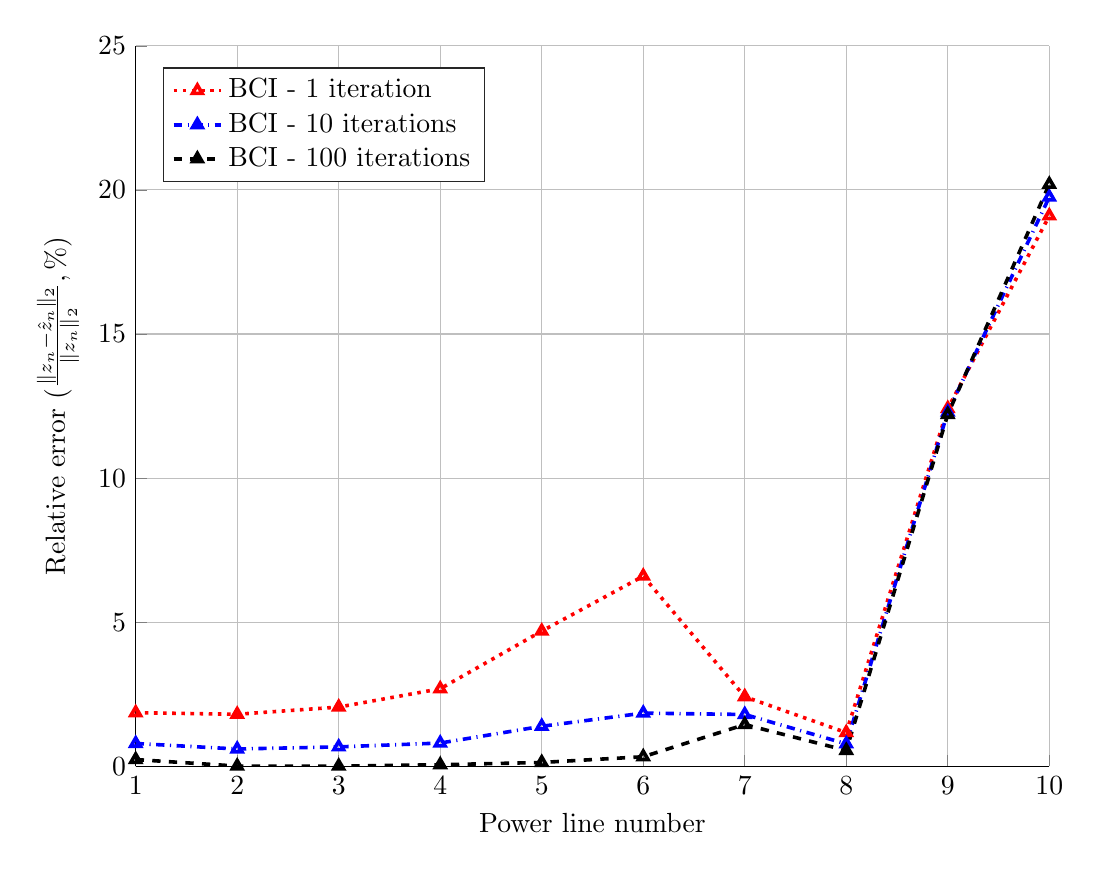
\begin{tikzpicture}

\begin{axis}[%
width=4.568in,
height=3.603in,
at={(0.766in,0.486in)},
scale only axis,
xmin=1,
xmax=10,
xlabel={Power line number},
xmajorgrids,
ymin=0,
ymax=25,
ylabel={Relative error ($\frac{\|z_n - \hat{z}_n\|_2}{\|z_n\|_2}, \%$)},
ymajorgrids,
axis background/.style={fill=white},
axis x line*=bottom,
axis y line*=left,
legend style={at={(0.03,0.97)},anchor=north west,legend cell align=left,align=left,draw=white!15!black}
]
\addplot [color=red,dotted,line width=1.3pt,mark=triangle,mark options={solid}]
  table[row sep=crcr]{%
1	1.86282972853486\\
2	1.80974930210926\\
3	2.05876660922205\\
4	2.69288038771469\\
5	4.69284271965727\\
6	6.60078620858525\\
7	2.4183047512369\\
8	1.17229841377977\\
9	12.4156099162367\\
10	19.1012714064646\\
};
\addlegendentry{BCI - 1 iteration};

\addplot [color=blue,dashdotted,line width=1.3pt,mark=triangle,mark options={solid}]
  table[row sep=crcr]{%
1	0.795804017958686\\
2	0.604226194957289\\
3	0.677257290769039\\
4	0.810692828095033\\
5	1.39230210574425\\
6	1.84859803736056\\
7	1.8015597080354\\
8	0.783048048146569\\
9	12.2918230336257\\
10	19.7526223259442\\
};
\addlegendentry{BCI - 10 iterations};

\addplot [color=black,dashed,line width=1.3pt,mark=triangle,mark options={solid}]
  table[row sep=crcr]{%
1	0.2379258512066\\
2	0.011802183091728\\
3	0.00988050495371802\\
4	0.0575283696697083\\
5	0.137383118634433\\
6	0.335269953928139\\
7	1.45159908543295\\
8	0.553975775571669\\
9	12.2105917660143\\
10	20.1957499220109\\
};
\addlegendentry{BCI - 100 iterations};

\end{axis}
\end{tikzpicture}%
\end{document}